\chapter{\telemacsystem development plan}
\label{devplan}

The development plan describes explicitly all the processes on the software
during the life cycle of the \telemacsystem code and insures its Quality of
the software.

The \telemacsystem activity is decomposed into three main activities from the creation of
a version, to its release and finally its removal:
\begin{itemize}
\item \textbf{Development activity}: Concerns any intervention on the source
code of \telemacsystem, its documentation, its associated tools may it be for a
corrective, adaptive or evolution maintenance.
\item \textbf{Verification and Validation activity}: Every development must go
through the verification and validation process. A major version must go
through the full validation before its release.
\item \textbf{Release activity}: Concerns the diffusion, support and maintenance
of the different versions of the code.
\end{itemize}

The development plan describes the action having a direct impact on the source
code. The other action are described in the SQP.

\section{Rights to commit new developments}

People intervening in the development of \telemacsystem can be divided in the following
groups:
\begin{itemize}
\item \textbf{The \telemacsystem development team (TDT)}: To be a part of the TDT you
need to have writing access on the subversion repository. To be in the
development team, the developer must have followed the \telemacsystem workshop and know
the SQP in order to apply it to its future developments. The PM is a member of
the TDT.
\item \textbf{Developers from EDF units}: They are developers from one of the
group of EDF and are developing for the \telemacsystem project. It is recommended that
they follow the \telemacsystem workshop. They will need to contact a member of the TDT
to integrate their development.
\item \textbf{Non EDF developers working with EDF}: They can be subcontractors,
interns, PhD students or any other partners working with EDF. It is also
recommended that they follow the \telemacsystem workshop. The follow-up of the
development will have to be made by a members of the TDT.
\item \textbf{Open source community, academic and industrial partners}: \telemacsystem
is an open source code under GNU-GPL. Anyone can get the source and develop his
own version. But for a development to be integrated in the official version, it
must be studied by the TDT and follow the process described in \ref{dev}. If the
integration is validated, the delivery of the evolution for the code must go
through a member of the TDT (See \ref{devint}).
\end{itemize}

\section{Life cycle of a development}

\subsection{Definition of a development}
\label{defdev}

A development represents a modification on the source code of \telemacsystem, its
documentation and its dedicated tools. (i.e. everything that is under the
configuration, see \ref{conf}). The developments are categorised in three types
of maintenance:
\begin{itemize}
\item \textbf{Evolution maintenance}: This maintenance aims to upgrade the
software in order to:
\begin{itemize}
\item Break limits of some existing functionalities (performance, strength,
precision...).
\item Develops new functionalities to satisfy new needs or demands. 
\end{itemize}
Those evolutions can be developments of new features made by one of EDF
Units. They can also originate from an outside developer and been brought in
by the PM.
Every maintenance must be joined with a CUE ticket. This ticket will allow the PM
to have a general view of the work in progress in the code. According to the
size of the development, it can even be presented by the developer in an ADEPHE
meeting, this will allow the TDT do evaluate the impact of the development and
maybe advice the developer on what to do. The development must be validated by
one of the CHs.
\item \textbf{Corrective maintenance}: The corrective maintenance is the removal
of an anomaly in the code or the documentation. A bug can be:
\begin{itemize}
\item A problem in the code, a mistake in the documentation, an error in
the GUI.
\item An error in a test case detected during the Verification and Validation
process.
\item A problem in the implementation detected by user.
\end{itemize}
Corrective maintenance must also be coupled with a CUE ticket.
\item \textbf{Adaptive maintenance}: The adaptive maintenance concerns evolution
in the code to comply with a change of environment (Operating System, compiler,
new cluster \ldots).
\end{itemize}

Each of those activities will be tied to a CUE ticket. The Type of CUE Ticket
will be determined by the kind of activity (Bug, Feature, Documentation...).
Every bug ticket should be resolved before the release of a new version.


\subsection{Life cycle of a \telemacsystem development}
\label{lifecycle}
The life cycle of a \telemacsystem development follows a list of 7 steps shown on the
Figure \ref{cycle}. Those steps will be described in the next section.

\begin{figure}[H]
\centering
\begin{tikzpicture}[node distance = 1cm, auto]
  % Defining style for the task
  \tikzstyle{task} = [draw, very thick, fill=white, rectangle]
  \tikzstyle{bigbox} = [draw, thin, rounded corners, rectangle]
  \tikzstyle{box} = [draw, thick, fill=white, rounded corners, rectangle]
  % Creation of the nodes
  \node (CUE) [task] {1. Ticket on CUE};
  \node (CHs) [task, below of=CUE] {2. CHs}; 
  \node (ADEPHE) [task, below of=CHs] {3. ADEPHE}; 
  \node (IMPL) [task, below of=ADEPHE] {4. Implementation}; 
  \node (null2) [right of=IMPL, node distance=9em] {};
  \node (VV) [task, below of=IMPL] {5. Verification \& Validation}; 
  \node (DOC) [task, below of=VV] {6. Documentation}; 
  \node (INT) [task, below of=DOC] {7. Integration "ADEPHE"}; 
  \node (null1) [right of=INT, node distance=9em] {};
  \node (null3) [left of=INT, node distance=9em] {};
  \node (TRUNK) [box, below of=INT, node distance=4em] {Main branch of \telemacsystem};
  \node (VALID) [task, below of=TRUNK] {Full validation};
  \node (TAG) [box, below of=VALID] {Release of \telemacsystem (tag)};
  % big box
  \node (DEV) [bigbox, fit = (CUE) (CHs) (ADEPHE) (IMPL) (null1) (null2) (null3) (VV) (DOC) (INT)] {};
  \node at (DEV.north) [above, inner sep=3mm] {\textbf{Development}};
  % Creation of the path between the nodes
  \draw[->] (CUE) to node {} (CHs);
  \draw[->] (CHs) to node {} (ADEPHE);
  \draw[->] (ADEPHE) to node {} (IMPL);
  \draw[->] (IMPL) to node {} (VV);
  \draw[->] (VV) to node {} (DOC);
  \draw[->] (DOC) to node {} (INT);
  \draw[-] (INT) -- node [near start] {no} (null1.center);
  \draw[-] (null1.center) -- (null2.center);
  \draw[->] (null2.center) -- node [near start] {} (IMPL);
  \draw[->] (INT) to node {yes} (TRUNK);
  \draw[->] (TRUNK) to node {} (VALID);
  \draw[->] (VALID) to node {} (TAG);
\end{tikzpicture}
\caption{\label{cycle}Life cycle of a \telemacsystem development}
\end{figure}

Depending on the kind of development (corrective, adaptive, evolution
maintenance) some of those steps can be skipped.
The different steps are:
\begin{enumerate}
\item Proposal step.
\item Job repartition step.
\item Examination and impact study step.
\item Implementation step.
\item Verification step.
\item Documentation step.
\item Approbation and validation step.
\end{enumerate}

This development cycle is based on a V scheme life cycle, it contains those
different steps and the different types of testing (See next paragraph). To be
more precise it is more of spiral cycle in which the V cycle is read
iteratively in order to improve the quality gradually. 

\section{Description of the development steps}
\label{dev}

\subsection{Proposal step}

Every demand must go through the proposal step may it be a corrective,
adaptive, evolution maintenance (See section \ref{defdev} for a definition).

This proposal is given to the TDT with a ticket on the CUE (\url{cue.opentelemac.org}).

The goal of this proposal is to:
\begin{itemize}
\item Inform the CHs of the development proposed.
\item Give more information on the impact study.
\item Plan and organise the resources for the development.
\item To prepare the validation in ADEPHE if necessary.
\end{itemize}

\textbf{In charge}: The proposer.

\textbf{Documents}: The CUE ticket.

\subsection{Job repartition step}
The job repartition step is made by the CHs in collaboration with the PM.
\begin{itemize}
\item If the proposal is not in a specific project, the CHs can propose to have
it billed by the \telemacsystem project. If the proposal is specific to a work project
the CHs can transfer the proposal to that project, if the proposal is
transfered the same tools (CUE, CIS...) will be used by the new project.
\item If the proposal is bound to a project, the resources for the development
will come from that project, the \telemacsystem project can still allocate some
resources in order to help, guide and give advice to the developer.
\end{itemize}

\textbf{In charge}: The CHs.

\textbf{Documents}: Update of the CUE ticket.

\subsection{Examination and impact study step}

When the cue ticket is published, the CHs have to determine if the development
must be followed by the TDT and presented in ADEPHE. This mainly concerns
evolution maintenance but can also concern corrective maintenance if it has a
major impact on the code.

The goal of the study impact is:
\begin{itemize}
\item If it is a evolution maintenance, to verify the coherence of the
evolution with: the kernel, the existing, in development or planned
functionalities, the functionality itself, the modifications needed in the
data structure, the architecture of the code or the GUI, the name of the new
keywords and structure. In particular guiding the developer towards a reusing
of existing routines.
\item In case of a corrective maintenance it studies the impact on the GUI and
the validation and Verification process.
\item To help the developer in its choice of algorithm and implementation.
\item To discuss the test cases for Validation and Verification.
\item To estimate the impact on the documentation.
\end{itemize}

If the development is heavy on the code, multiple ADEPHE can be used to follow
the development.


\textbf{In charge}: CHs, TDT, handler of the development.

\textbf{Documents}: 
\begin{itemize}
\item INPUT: The CUE ticket.
\item OUTPUT: Reports after each ADEPHE.
\end{itemize}


\subsection{Implementation step}

This is the coding part of what was specified in the CUE ticket, with the
modifications that the discussion during the ADEPHE could have generated.

The developer must follow the coding convention given in the developer guide of
\telemacsystem (Available in Appendix \ref{codingconv}). All the developments are made
under a configuration handling tool (SVN), for each development a branch is
created dedicated to that development.

The control of the implementation is made through tests:
\begin{itemize}
\item Evolution maintenance:
\begin{itemize}
\item Unit tests (Non-exhaustive list):
\begin{itemize}
\item Parallelism testing.
\item Continued computation testing.
\item Post-treatment testing.
\item GUI testing.
\end{itemize}
\item Verification test: one or more depending of what is proposed by the
developer (seen in ADEPHE, if there was one).
\item Validation test: one or more depending of what is proposed by the
developer (seen in ADEPHE, if there was one).
\end{itemize}
\item Corrective or adaptive maintenance:
\begin{itemize}
\item Old unit test if impacted.
\item Verification and validation test.
\end{itemize}
\end{itemize}

The Unit tests are for the developer to create.

The development must be made on a branch and follow the development version
(or trunk, see Section \ref{conf} for a definition) using a configuration
handling tool (SVN is used in Edf). It is strongly recommended to keep up to
date with the development version as often as possible. This lessens the
workload of that process compared to doing it at the end of the development.
The Figure \ref{fig_feature} shows what the evolution of the development should
look like.

\begin{figure}[H]
\centering
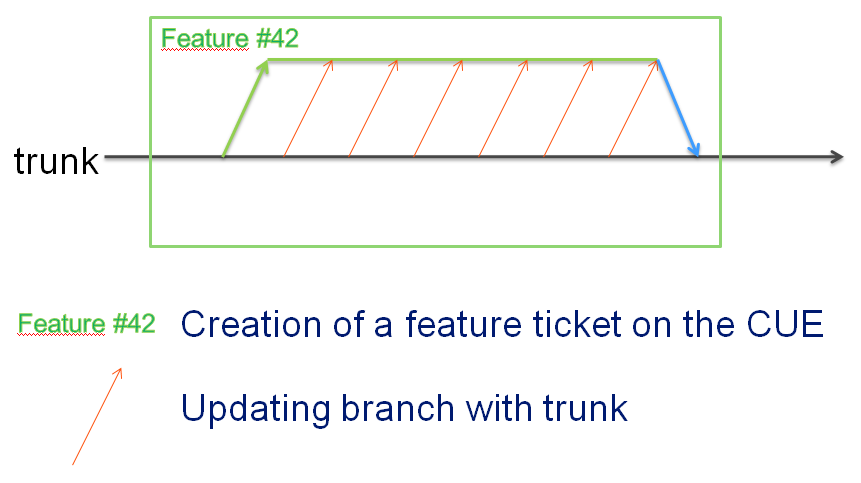
\includegraphics[scale=.4]{graphics/feature_svn.png}
\caption{\label{fig_feature} Life cycle of a development branch}
\end{figure}

It is also recommend to use developing tools during the development like a
debugger (gdb, totalview), valgrind for memory leak.

Every development must be tested both in serial and parallel configuration and
the GUI must be updated accordingly.

The CUE ticket is updated as the implementation goes on.

\textbf{In charge}: The developer.

\textbf{Documents}: 
\begin{itemize}
\item INPUT: cue ticket, developer manual, verification and validation test cases.
\item OUTPUT: source code, test cases (with xml), result of tests.
\end{itemize}

\subsection{Verification step}

The Verification and Validation process is deeply linked with the
implementation process. This process aims to verify the code on the algorithm
level and the whole model using the validation and verification test cases
(even if a small part of the code was modified like during a corrective and
adaptive maintenance). This is then complementary (even redundant) with the
verification done during the implementation.  The verification and validation
as distinguish as describe below:
% Copy of what is in organisation.tex subsection{Verification and validation activity}
\begin{itemize}
\item \textbf{Verification}: The verification aims to establish that the code
solves efficiently the mathematical problem he is supposed to resolve (and that
is described in the specification of the concern algorithm). The verification
focuses on the quality of the implementation from a computer science and
theoretical point of view. The answer to the verification process is a binary
one: the code does or does not respond to the demands. To do that the
verification is using an analytical solution of the model or a solution based
on measurements with the possible addition of source terms to the equation. The
process is then most of the time to compared the numerical solution with a
reference solution on meshes with increasing mesh refinement. This verifies
that the algorithm converges in mesh and gives the level of precision
associated.
\item \textbf{Validation}: The validation aims to see to what level the code is
able to answer to a physical problem in a given application domain.  The
validation focuses on the ability of the code to predict event from a physical
point of view. The answer to this process is not binary. The evaluation is made
through a comparison between a numerical solution and an experimental solution.
We distinguish the validation with separated effects, which focuses on an
isolated physical phenomenon and the full validation which focuses on an
industrial problem (which can be simplified to get access to experimental
measurements) composed of multiple physical phenomenon.
\end{itemize}

As mentioned in the previous paragraph every development must contain
validation and verification test cases:
\begin{itemize}
\item Evolution maintenance: For an evolution of the code at least one
verification and one validation case must be added if existing cases can not be
used. The choice of those cases are discussed in ADEPHE.
\item Corrective and adaptive maintenance: All the test cases must be rerun.
\end{itemize}

\textbf{In charge}: The developer.

\textbf{Documents}:
\begin{itemize}
\item INPUT: cue ticket, validation manual, ticket for each case.
\item OUTPUT: update of cue ticket, \LaTeX\xspace documentation follow the validation
standard for each test case.
\end{itemize}

\subsection{Documentation step}

The \telemacsystem technical documentation is composed of the following manuals:
\begin{itemize}
\item \textbf{Reference Manual}: describes every keyword in the dictionary of
one module.
\item \textbf{Principle Note}: describes the physical phenomena modelled by the
module and the numerical methods used to solve the equations modelling these
phenomena.
\item \textbf{Validation Manual}: presents a list of test cases which validate
the conceptual model, algorithms and software implementations. It is a
concatenation of all the test case documentation for one module.
\item \textbf{User Manual}: describes how to use the code.
\item \textbf{Release Note}: lists the new features of the version.
\item \textbf{Environment Guide}: gives a list of the environment commands.
\item \textbf{Online Manual(Doxygen)}: This documentation is linked with the
source code (it is build by using special comment made in the source code), it
describes the functions and structures of the source code.
\item \textbf{Installation Manual}: describes the process to follow to install
the \telemacsystem code.
\item \textbf{Developer Manual}: describes all the actions a developer might have
to do during a development it also defines the programming convention.
\end{itemize}

The first five manuals are duplicated for each of the modules of \telemacsystem.  The
documentations are under configuration handler (svn) in \LaTeX\xspace format.  The last
two documentation are available on the \telemacsystem website.  The documentation is
under the responsibility of the Doc Handler and the CHs.

Depending on the type of development a few cases can occur:
\begin{itemize}
\item \textbf{Evolution Maintenance}: For a new functionality of the code, a
new section must be added in the principle note describing the new physics and in
the user manual showing how to use that functionality. The Online documentation must
be updated as well.
\item \textbf{Corrective, adaptive Maintenance}: If the development has an
impact on the documentation, it must be updated by the developer.
\end{itemize}

In any case the modification must go through the Doc Handler and must be
validated by the CHs and the PM.

\textbf{In charge}: The Doc Hand.

\textbf{Documents}:
\begin{itemize}
\item INPUT: All the documentation.
\item OUTPUT: The updated documentation.
\end{itemize}

\subsection{Integration step}

The integration step concerns the restitution of a development into the
main branch of \telemacsystem (trunk, see \ref{conf}).

The integration step is composed of at most 4 steps, the presentation in ADEPHE
being optional:
\begin{itemize}
\item Demand for a presentation in ADEPHE, the demand is made through the CUE
ticket.
\item Presentation of the development and the verification case in ADEPHE.
\item Designing the member of the TDT in charge of the integration of the
development.
\item Integration of the verification and validation cases under the
supervision of the V\&V Hand.
\end{itemize}

Not following those steps allows the CHs to refuse the integration and even
remove it from the development version. We describe below the presentation in
ADEPHE and the integration process.

\textbf{Presentation of the development in ADEPHE}

The ADEPHE meeting are bi-monthly.
Must go to an approbation in ADEPHE:
\begin{itemize}
\item Any evolution maintenance out of the \telemacsystem project.
\item Important modification in the code with the approbation of the CHs.
\end{itemize}

To be allowed in ADEPHE, a developer must have:
\begin{itemize}
\item Synchronize its branch with the latest version of the main branch
(trunk).
\item Verify that the code follows the programming rules and that the unit test
are working.
\item The new test cases added by the development must pass through the
validation tool (CIS).
\item Update the CUE ticket.
\end{itemize}

During the ADEPHE the person in charge of the development must present:
\begin{itemize}
\item The development and how it was implemented: the functionalities if it is a
evolution maintenance, in case of a corrective, adaptive
maintenance: the data structure, the new keywords, how to use it.
\item The modifications in the GUI if they are any.
\item The verification and validation cases and their results.
\item The impact on the documentation.
\end{itemize}

At the end of the presentation the TDT must decide:
\begin{itemize}
\item The integration or the dismissal of the development in the trunk.
\item The integration or the dismissal of the test case.
\item The integration or the dismissal of the modifications on the
documentation.
\item The person in charge of the integration.
\end{itemize}

In case of a disagreement in the TDT the CHs have the final word.

\textbf{In charge}: CHs, TDT.

\textbf{Documents}:
\begin{itemize}
\item INPUT: CUE ticket, documentation.
\item OUTPUT: ADEPHE report, update of cue ticket.
\end{itemize}

\textbf{Integration}

After the ADEPHE meeting the person in charge of the integration has to do the
following actions:
\begin{itemize}
\item Integrate the verification and verification cases in the cases database. 
\item Push the development and the documentation modifications into the \telemacsystem
main branch.
\item Close the CUE ticket.
\end{itemize}

\textbf{In charge}: TDT.

\textbf{Documents}:
\begin{itemize}
\item INPUT: CUE ticket.
\item OUTPUT: update of CUE ticket, documentation updated.
\end{itemize}

\section{Maintenance}

In this part the maintenance concerns only the corrective and adaptive maintenance.

The \telemacsystem project is in charge of the non-regression of the \telemacsystem
functionalities on the Verification and Validation test base. 

The \telemacsystem project is also in charge of the adaptive maintenance (see Section
\ref{defdev}).

The project in charge of other developments is in charge of the corrective
maintenance for their developments. But an help from the TDT is possible in
case of big difficulties. If the bug is easy to correct the TDT can, with the
authorisation of the person on charge, correct the bug themselves.

In any case the development must follow the development step described in
section \ref{lifecycle} and summarised in Figure \ref{cycle}.

\textbf{Removal of a functionality}

The CHs can decide to remove a functionality if it has become obsolete or
irrelevant. This decision must be validated by the PM. The CHs must warn the
user community.

The removal of a functionality can only happen on the trunk, it is not
retroactive. 

The removal of a functionality concern:
\begin{itemize}
\item The source code and the library linked.
\item If there are any, the verification and validation impacted.
\item The documentation.
\item The GUI.
\end{itemize}

\section{Integration of development from the open-source community}
\label{devint}

The \telemacsystem project (CHs and PM) is in charge of the evaluation of development
from the open source community.

Two cases can occur:
\begin{itemize}
\item A CUE ticket is posted.
\item A member or entity of the open source community has developed a new
functionality and wants it to be included in the official version maintained by
EDF. A CUE ticket could have been made. 
\end{itemize}

To be a potential candidate for an integration in the development version of
\telemacsystem, a development from the open source community must:
\begin{itemize}
\item Be generic enough to be useful to the entire community. For example the
development must not be bound to an industrial application.
\item Impact as little as possible the structure of the code. And have a good
modularity so it can be deleted when the maintenance is not possible anymore.
\item Not be bound to a copyright, the code being under GNU GPL the development
must be under the same license.
\end{itemize}

If the development passes those three criteria then the integration is given to
a member of the TDT who becomes in charge of that development.

Then the development must follow the same processes, described in section
\ref{lifecycle}, as any other developments.

\section{Configuration handling}
\label{conf}

\subsection{Tools of configuration handling}

The different versions of the elements of the \telemacsystem software are handled by a
version control tool. Those tools allow to track the evolution and ease the
collaboration between multiple developers. Nonetheless, in addition to those
tools the source are saved on the EDF network NOE. 

The version control tool used is Subversion (SVN) which allows to rebuild any
version. The subversion repository is based at the following address:
\url{http://svn.opentelemac.org/svn/opentelemac}.

For each stable version a configuration note signed by the CHs and the RQ2 is published. It precises:
\begin{itemize}
\item The elements concerned.
\item The history of the configuration.
\item The organisation of spaces.
\item The creation of the stable version.
\item The saving and storing processes.
\end{itemize}

\subsection{Elements of the configuration}

The elements of the \telemacsystem software concerned by the configuration control are
given in the configuration note. 

The source code, the environment script, the documentation \ldots

\subsection{Type of version}

\textbf{\telemacsystem official or reference version}

An official (or reference) version is a version handled by the \telemacsystem project.
The official version are:
\begin{itemize}
\item The version out of exploitation.
\item The latest stable version, minor or major release.
\item The development version.
\end{itemize}

For example, the branch of development of the TDT are not considered
official.

\textbf{Creation of the reference version for \telemacsystem}

The creation of the reference version is described in the configuration note.
The process will be describe here as well:

The \telemacsystem version are handled using "tags".
\begin{itemize}
\item Creation a tag is decided by the Chain Hand. and the CHs.
\item Tags are created for every minor version.
\item Tags are named in the format \textbf{x.y.z} where:
\begin{itemize}
\item \textbf{x} is the major version index, incremented when a major
modification is made to the code (ex: makeover of the interface, modification
of the code structure...),
\item \textbf{y} is the minor version index, incremented when new minor
functionalities are added to the software,
\item \textbf{z} is the patch index, incremented when a group of bug
corrections are implemented in the software.
\end{itemize}
\end{itemize}

The version are divided into branches and tags. There is:
\begin{itemize}
\item \textbf{The main branch} (trunk), also called the development version. It
represents the work in progress between two stable version. It is where the
different maintenance are integrated. Figure \ref{fig_lifecycle} shows the
evolution of the main branch between two stable versions.
\item \textbf{The version branch} ($x.y$), they are created every new major or
minor version. They are used only for corrective and adaptive maintenance. They
have been through the complete validation process.
\item \textbf{The stable version tag} ($x.y.z$), the tags are made from the version
branch ($x.y$) those tags are fixed they will not be modified. If a corrective
or adaptive maintenance is necessary the changes will be made in the version
branch and a new tag ($x.y.(z+1)$) will be created. Figure \ref{minor_version}
shows the creation of the $x.y$ and the tags created.
\end{itemize}

\begin{figure}[H]
\centering
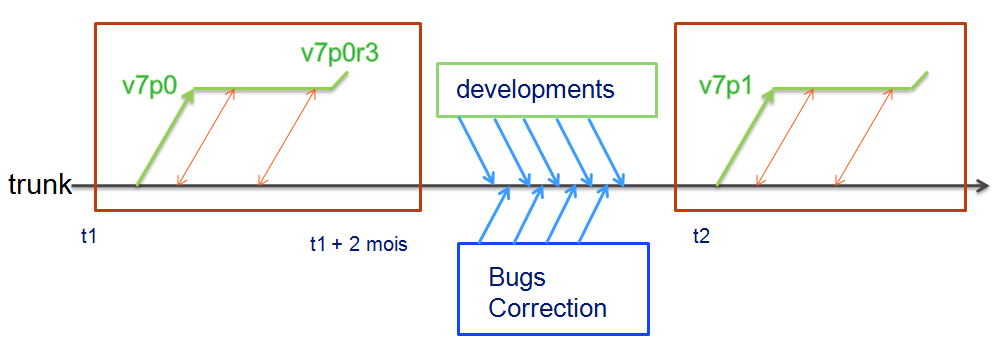
\includegraphics[scale=.4]{graphics/lifecycle.png}
\label{fig_lifecycle}
\caption{Life cycle of the \telemacsystem version}
\end{figure}

\begin{figure}[H]
\centering
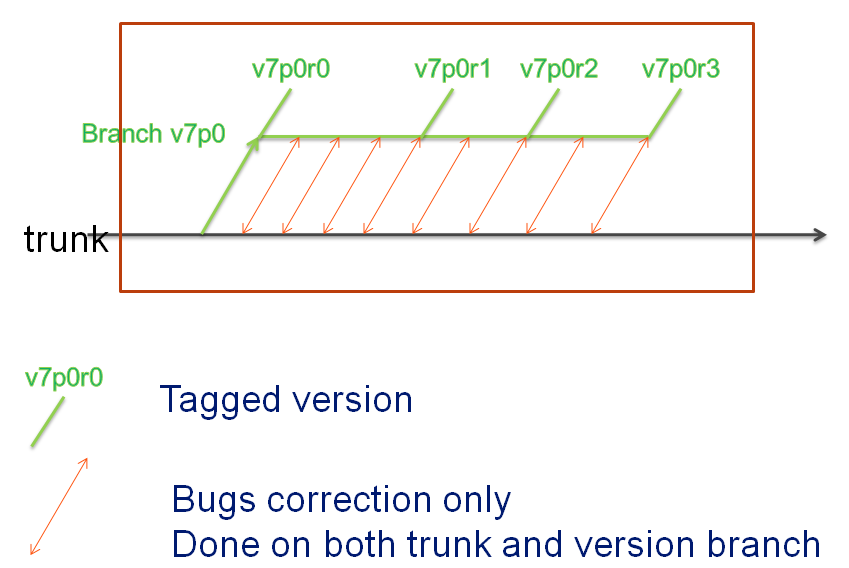
\includegraphics[scale=.4]{graphics/minor_version.png}
\caption{\label{minor_version} Life cycle of a version branch}
\end{figure}


Evolution maintenances are not merged on the version branch they are only
merged on the trunk.

\subsection{Version schedule}

\textbf{Version release}

The different version major and minor are separated by a flexible interval:
\begin{itemize}
\item The major version are out every 4-5 years.
\item The minor release are out every year, if the amount of new development is considered acceptable, and is maintained until the release
\end{itemize}

Finally at an instant $t$ in time we have the following version:
\begin{itemize}
\item The development version: It is the main branch (trunk).
\item The latest stable version $x.y.z$
\end{itemize}

This timetable can be modified due to a big change in the code that would
require longer validation to leave time for the normal integration to adapt.

\textbf{Removal of stable version}

The removal of a stable version is automatic when:
\begin{itemize}
\item A corrective version $z > 0$ is released.
\item It reaches its expiration date. 
\end{itemize}

\textbf{Version maintained}

Only last two minor version are maintained.

\textbf{Exploitation version}

To do a study with \telemacsystem it is recommended to use the latest stable version.
It should be the most advanced and least bugged version.
